\section{Remaining Figures}
\begin{figure}[h!]
    \centering
    \includegraphics[width=\textwidth]{bar_topics}
    \caption{
        Distribution of statements among the 9 topic categories divided into the assigned sentiment labels (-1:NEGATIVE, 0:NEUTRAL, 1:POSITIVE).
        A domination of neutral statements can be observed for each of the 9 topics.
        There are visibly more positive than negative statements except for Gaming and Machine Human Interface.
    }
    \label{fig:bar_topics}
    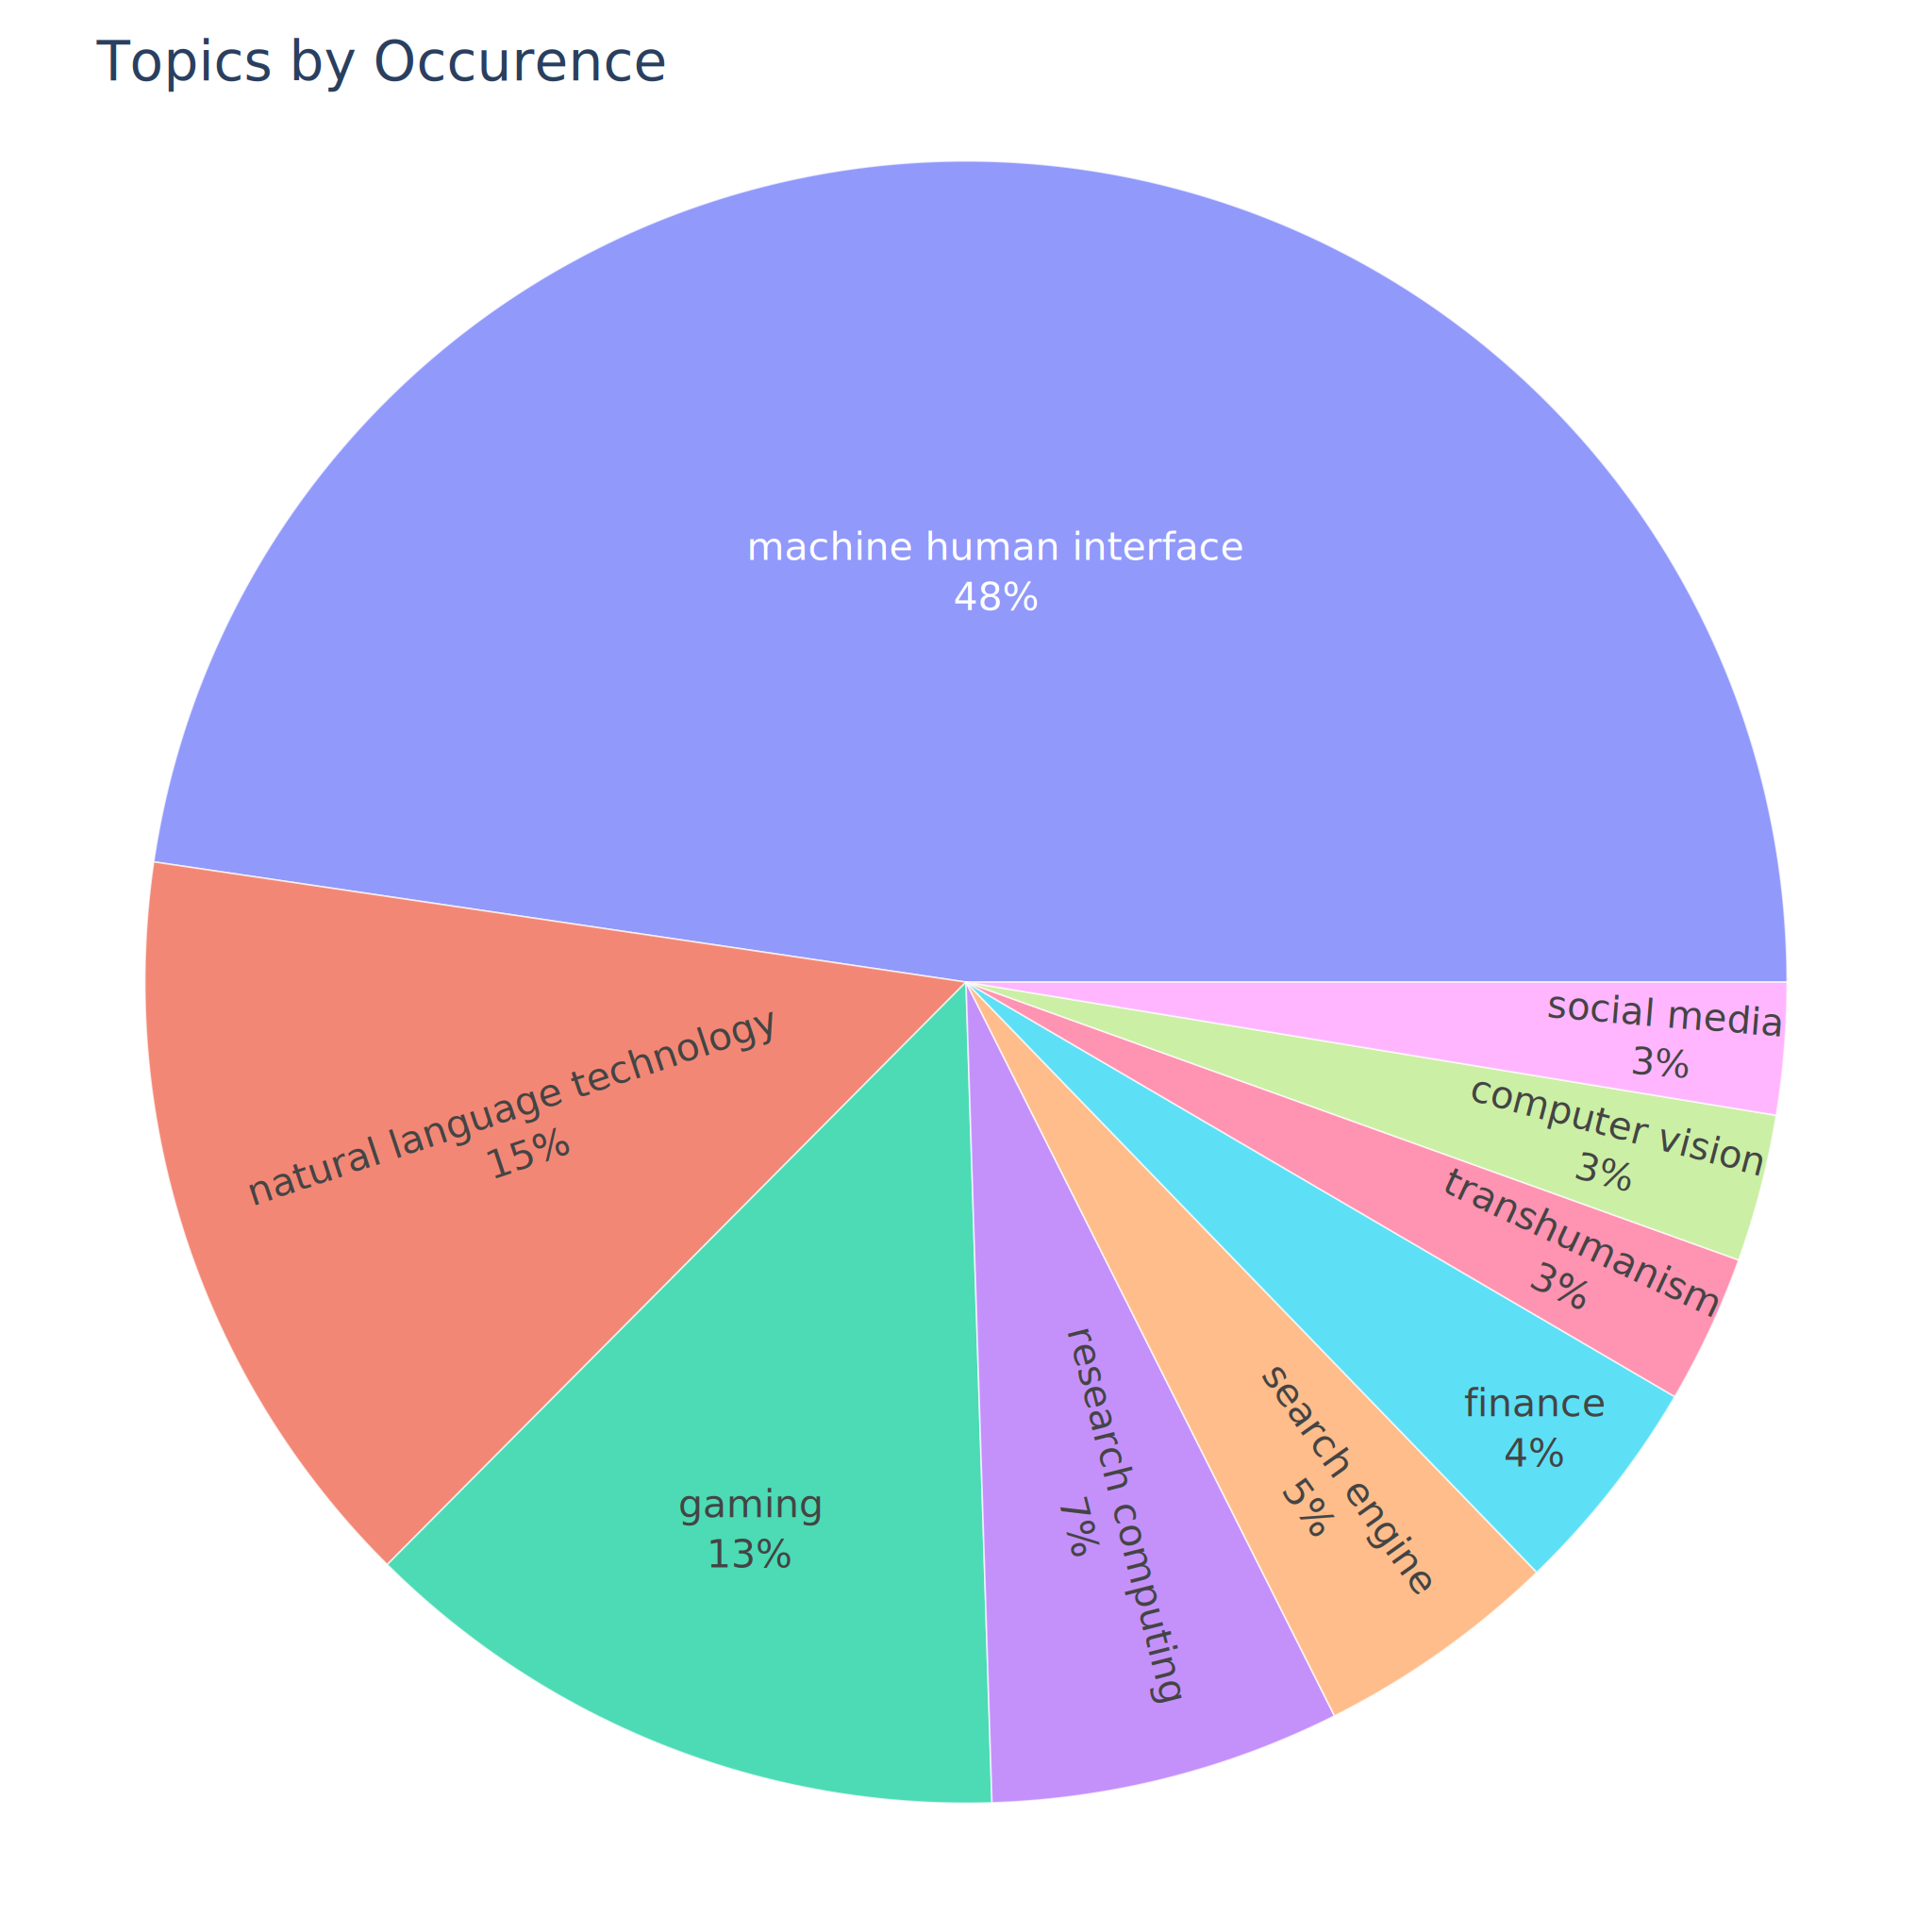
\includegraphics[width=0.6\textwidth]{pie_topics_by_occ}
    \caption{
        Distribution of statements among the 9 topic categories (in \%). 
        Statements are not equally distributed.
        Machine Human Interface describes about half of all statements (48\%).
        Gaming as well as Natural Language Technology account for about 15\% of all statements.
    }
    \label{fig:pie_topics_by_occ}
\end{figure}
\pagebreak
\begin{figure}[h!]
    \centering
    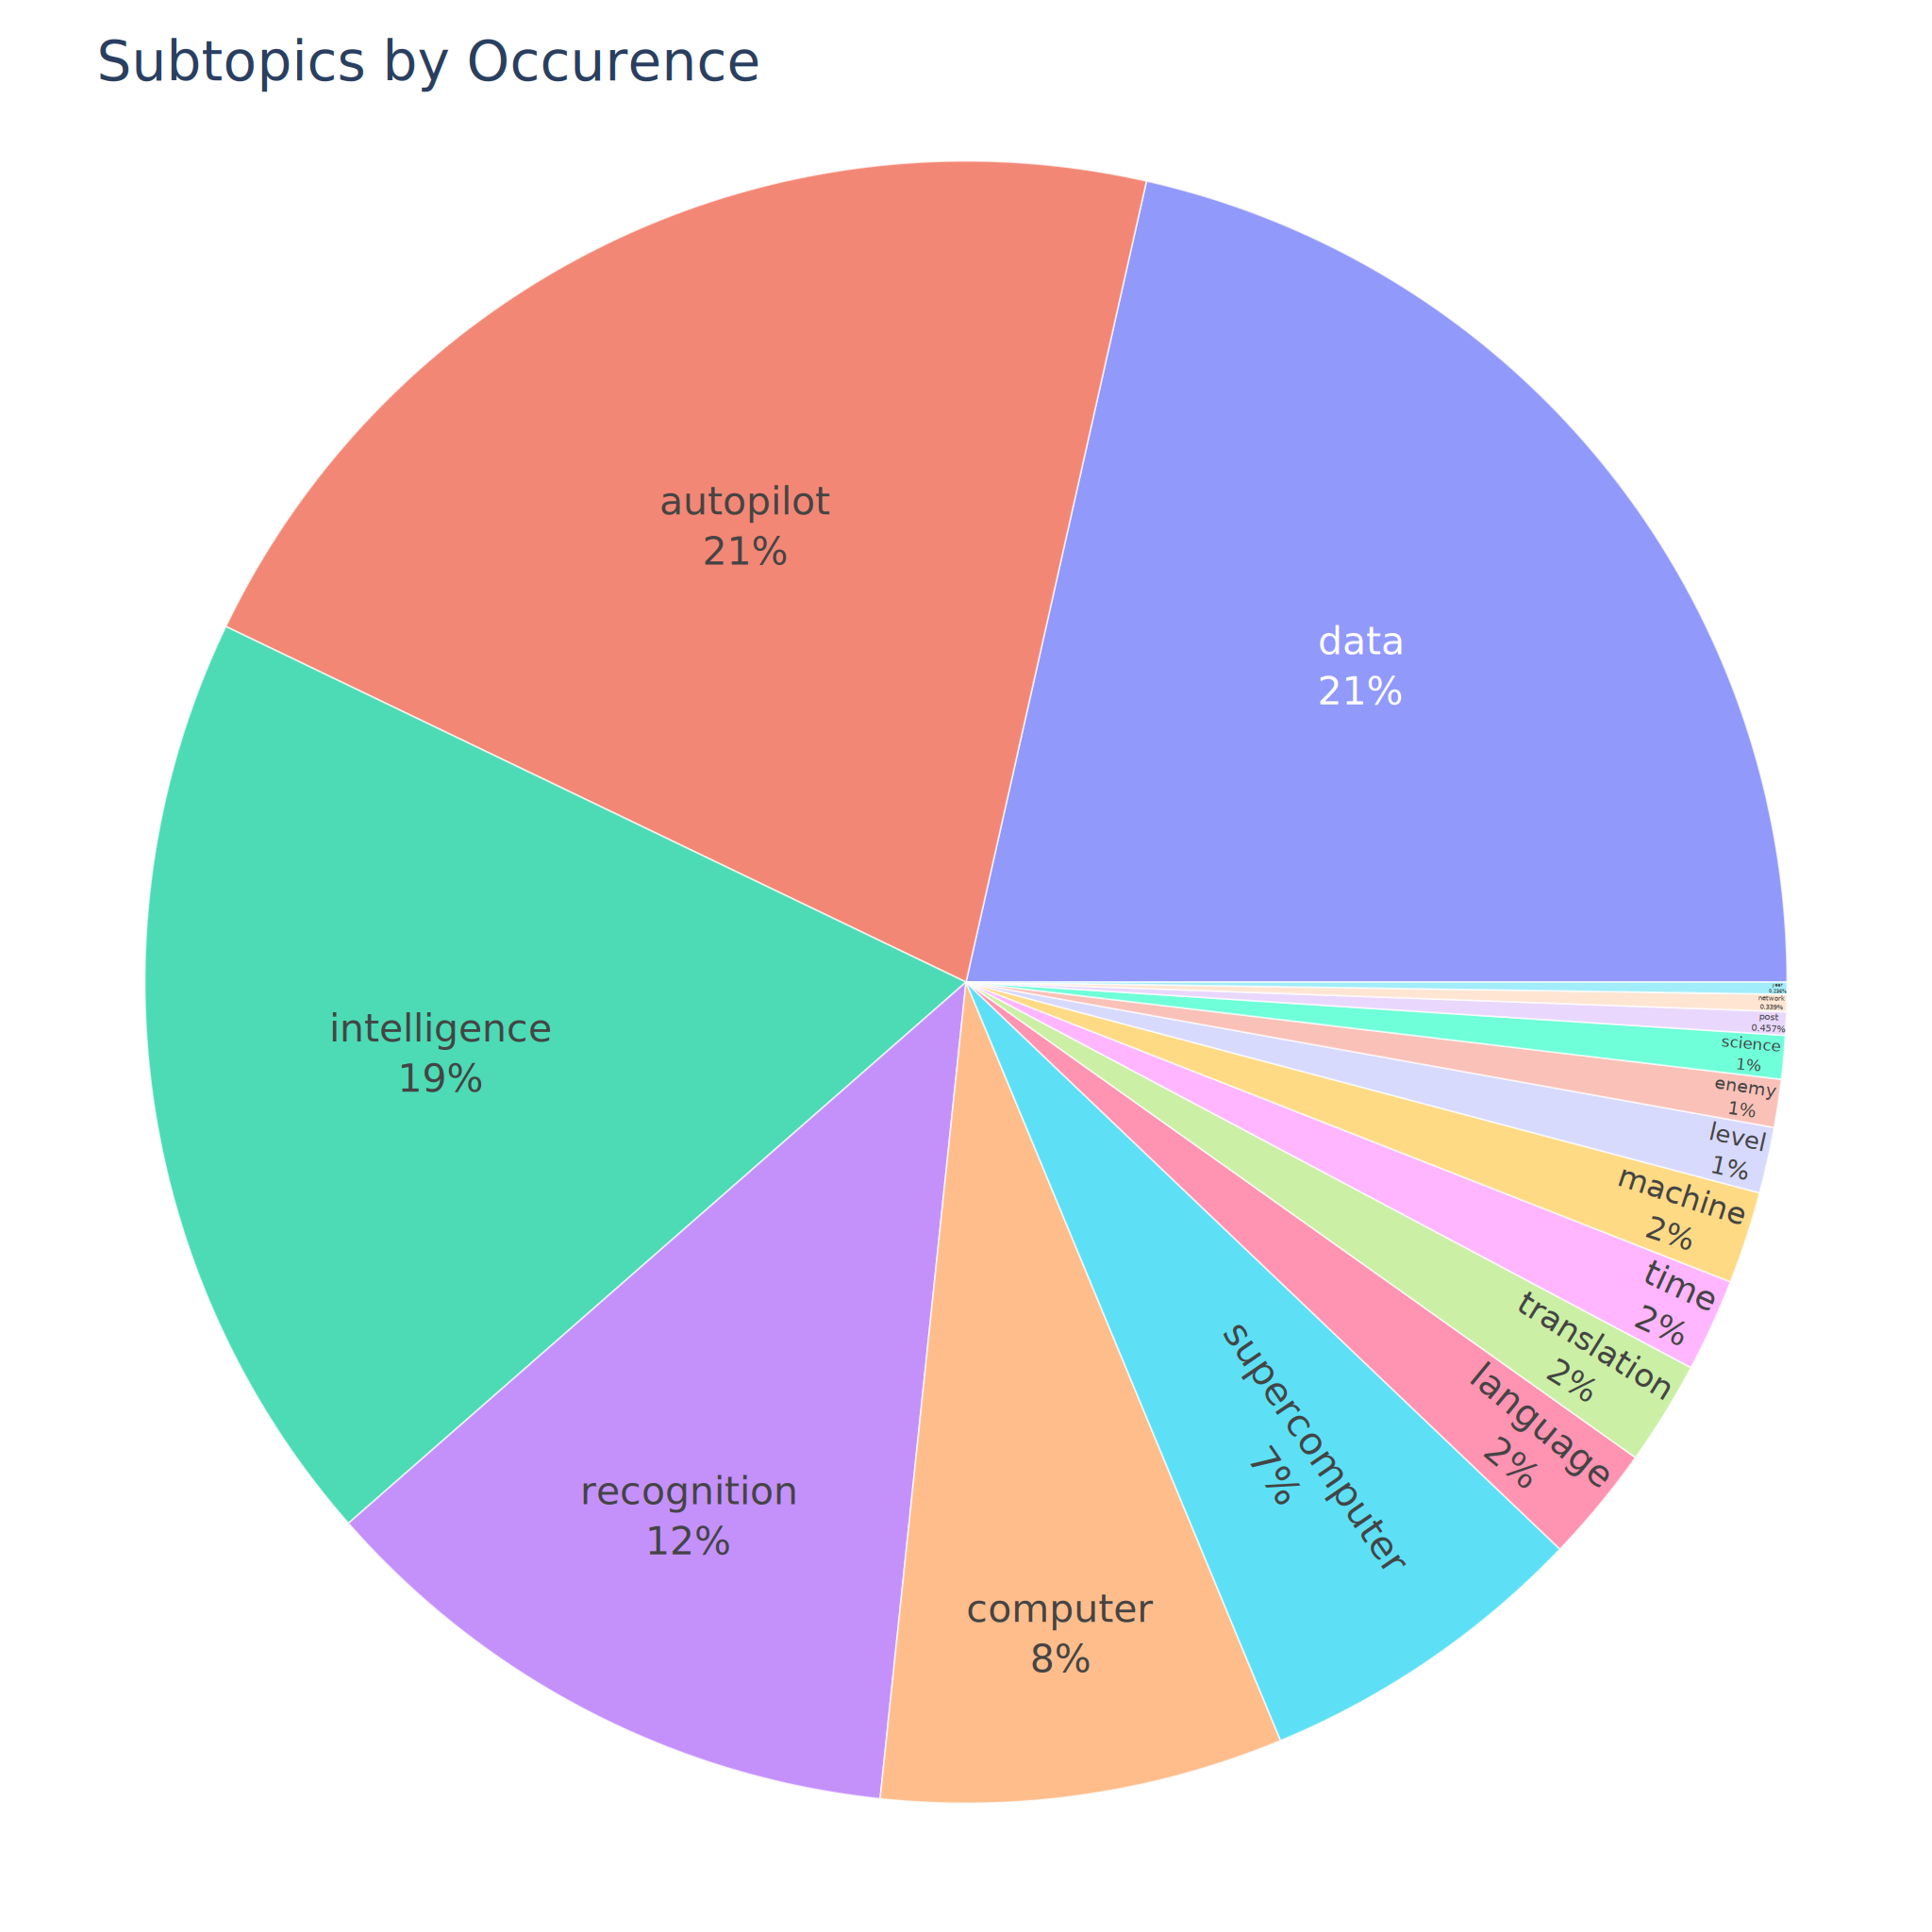
\includegraphics[width=0.6\textwidth]{pie_subtopics_by_occ}
    \caption{
        Distribution of statements among the most frequently occuring subtopic categories (in \%).
        Data (21\%), Autopilot (21\%) and Intelligence (19\%) are dominant subcategories.
    }
    \label{fig:pie_subtopics_by_occ}
    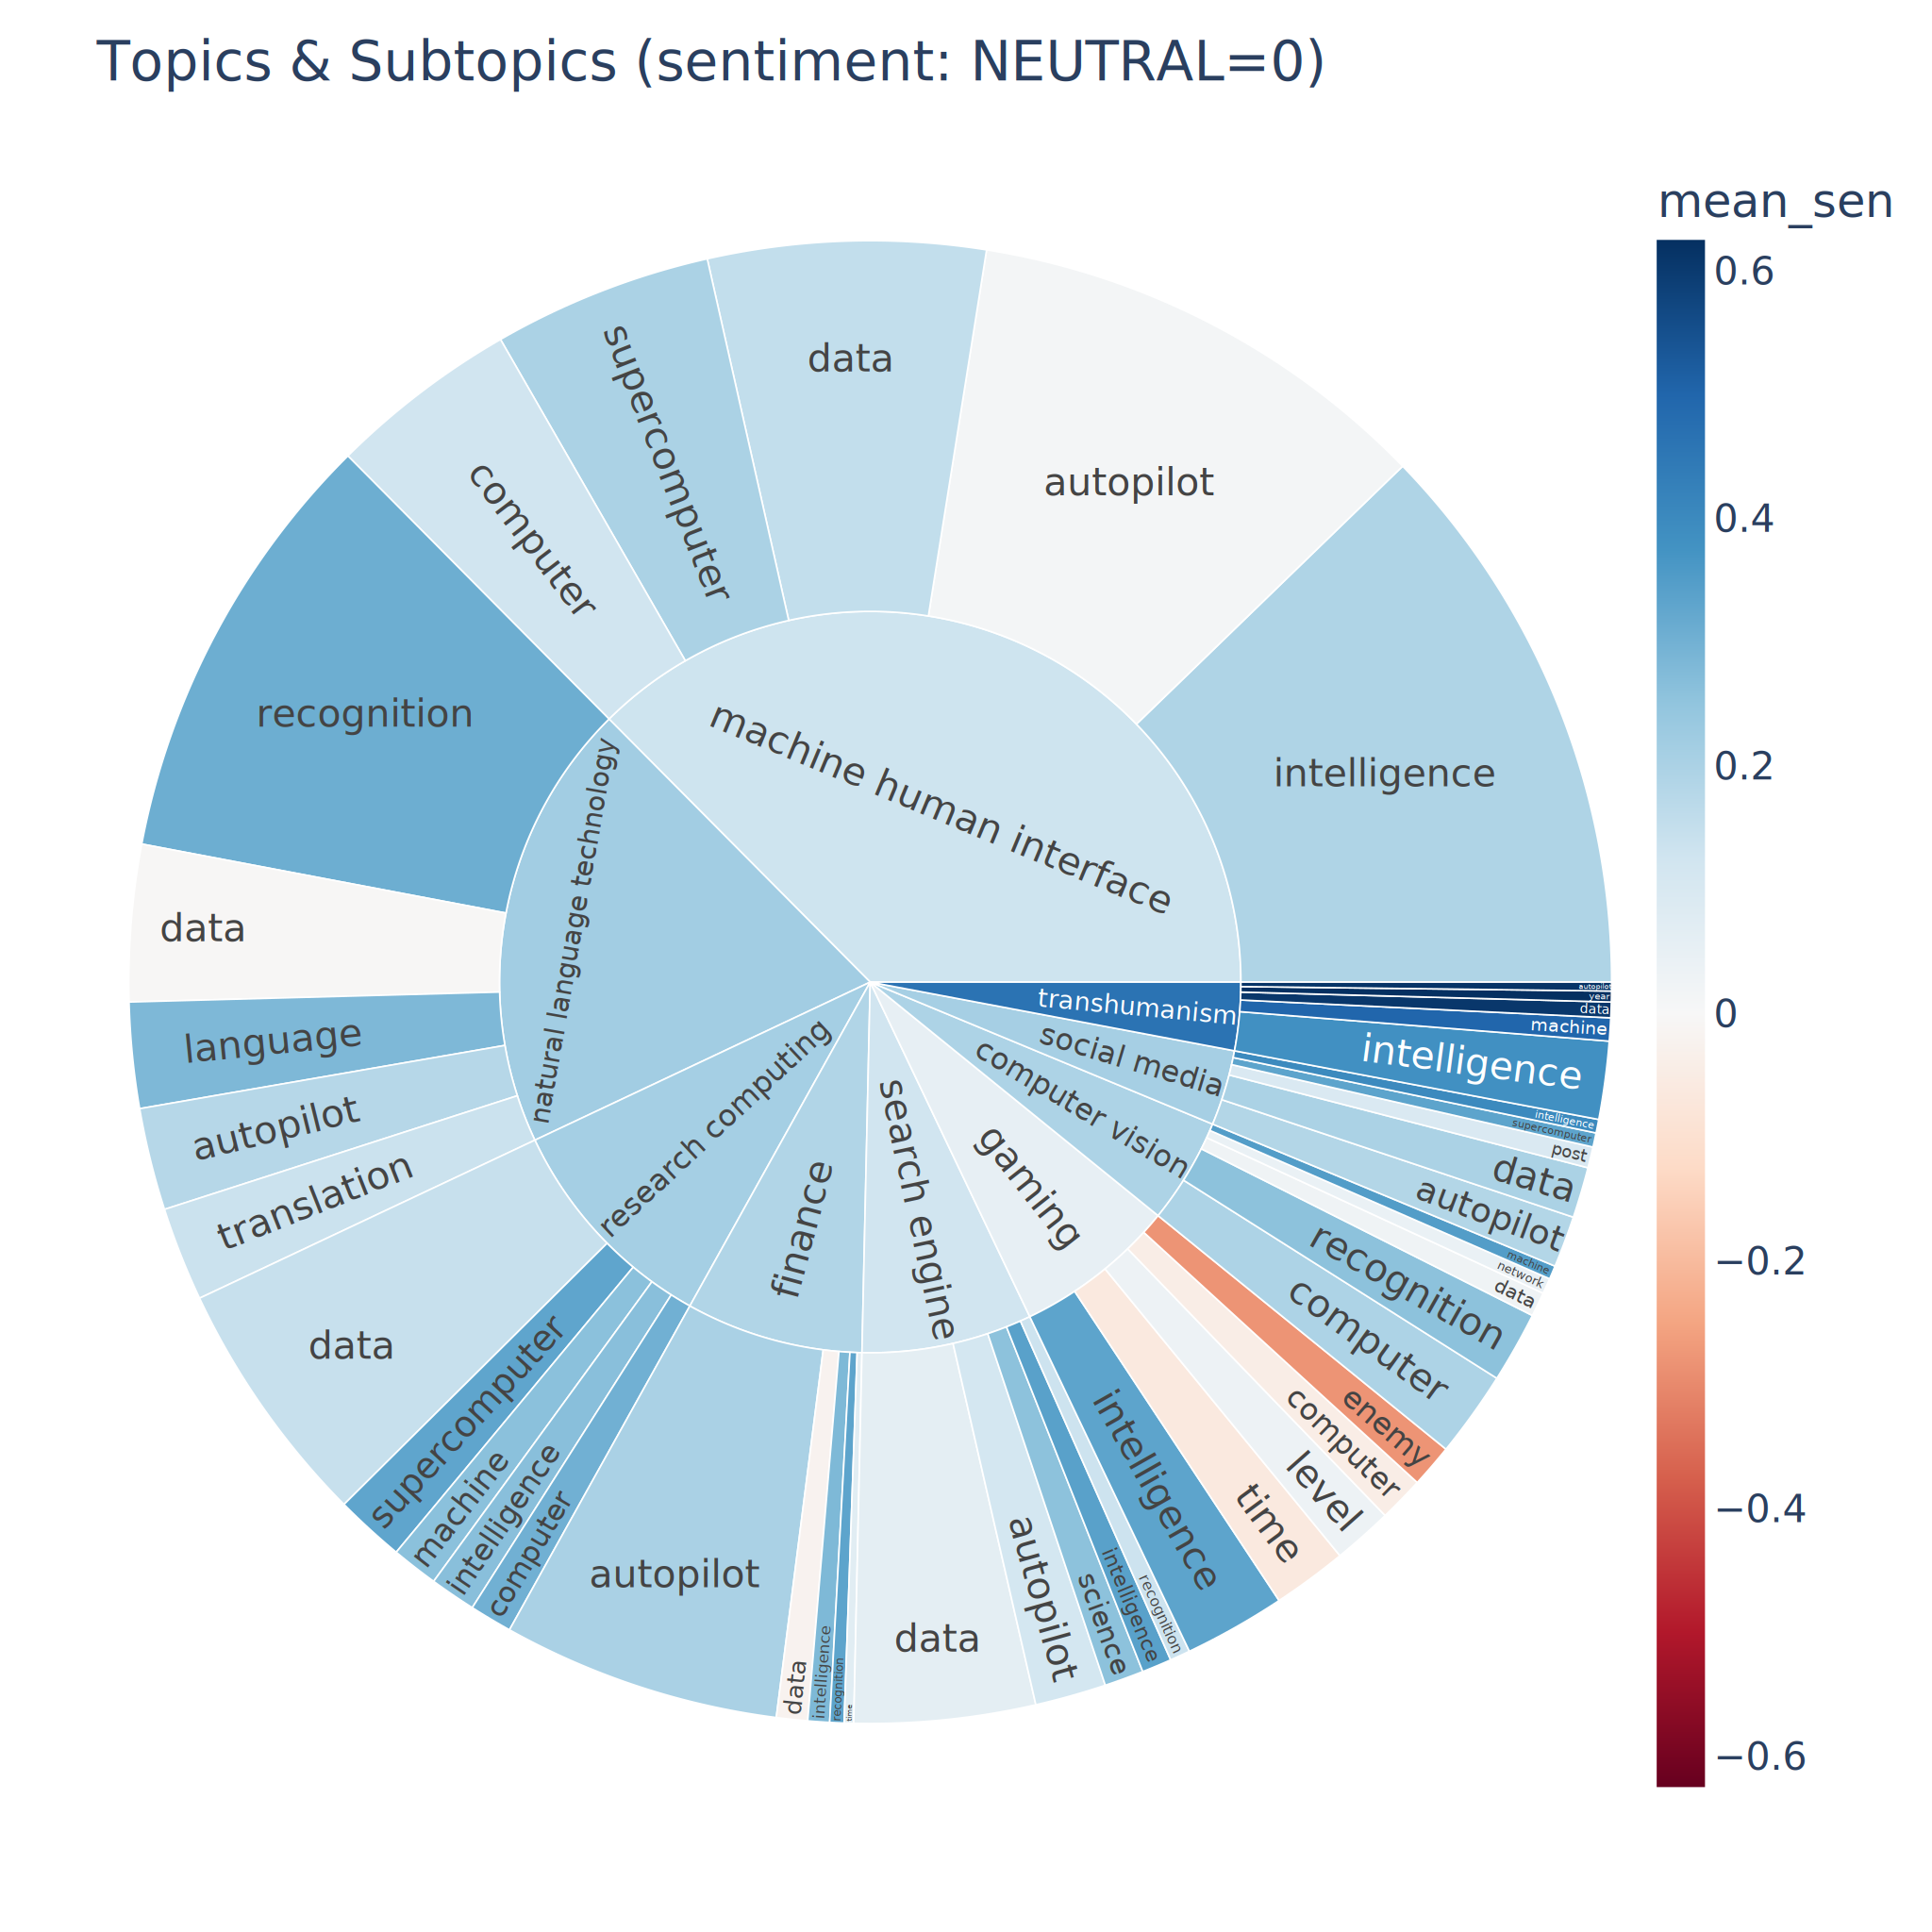
\includegraphics[width=0.6\textwidth]{pie_topics_subtopics_by_occ_sent_neu}
    \caption{
        Distribution of statements among the 9 topics (inner circle) and the most frequently occuring subtopic categories (outer circle).
        The Colorpalette (on the right) represents the average sentiment score of topics and subcategories (Red: NEGATIVE, White: NEUTRAL, Blue: POSITIVE).
        The majority of the average sentiment in both topics and subcategories is neutral.
    }
    \label{fig:pie_topics_subtopics_by_occ_sent_neu}
\end{figure}
